\documentclass[border=10pt]{standalone}
\usepackage{amsmath, amsfonts, amssymb, bm}
\usepackage{tikz}
\usetikzlibrary{shapes.geometric, arrows.meta, positioning, shadows.blur}
% Color and style setup
\definecolor{startcolor}{RGB}{255, 248, 240}
\definecolor{processcolor}{RGB}{240, 245, 255}
\definecolor{decisioncolor}{RGB}{245, 245, 245}
\definecolor{finalcolor}{RGB}{255, 240, 245}
\definecolor{arrowcolor}{RGB}{50, 50, 50}
\definecolor{yescolor}{RGB}{0, 100, 0}
\definecolor{nocolor}{RGB}{180, 0, 0}
\tikzset{
    font=\sffamily\bfseries,
    startstop/.style = {
        rectangle, rounded corners, minimum width=5cm, minimum height=1.2cm, 
        text centered, draw=arrowcolor, line width=1pt, fill=startcolor, blur shadow
    },
    block/.style = {
        rectangle, minimum width=5cm, minimum height=1.2cm, text centered, 
        text width=6.5cm, align=center, draw=arrowcolor, line width=1pt, fill=processcolor, blur shadow
    },
    decision/.style = {
        diamond, aspect=2.2, minimum width=5cm, minimum height=2.2cm,
        text centered, text width=4.75cm, align=center, draw=arrowcolor, 
        line width=1pt, fill=decisioncolor, inner sep=6pt, blur shadow
    },
    finalblock/.style = {
        rectangle, minimum width=5cm, minimum height=1.8cm, text centered, 
        text width=7cm, align=center, draw=arrowcolor, line width=1pt, fill=finalcolor, blur shadow
    },
    arrow/.style = {-{Stealth[length=4mm,width=2.5mm]}, ultra thick, draw=arrowcolor},
    yesarrow/.style = {arrow, draw=yescolor},
    noarrow/.style = {arrow, draw=nocolor}
}
\begin{document}
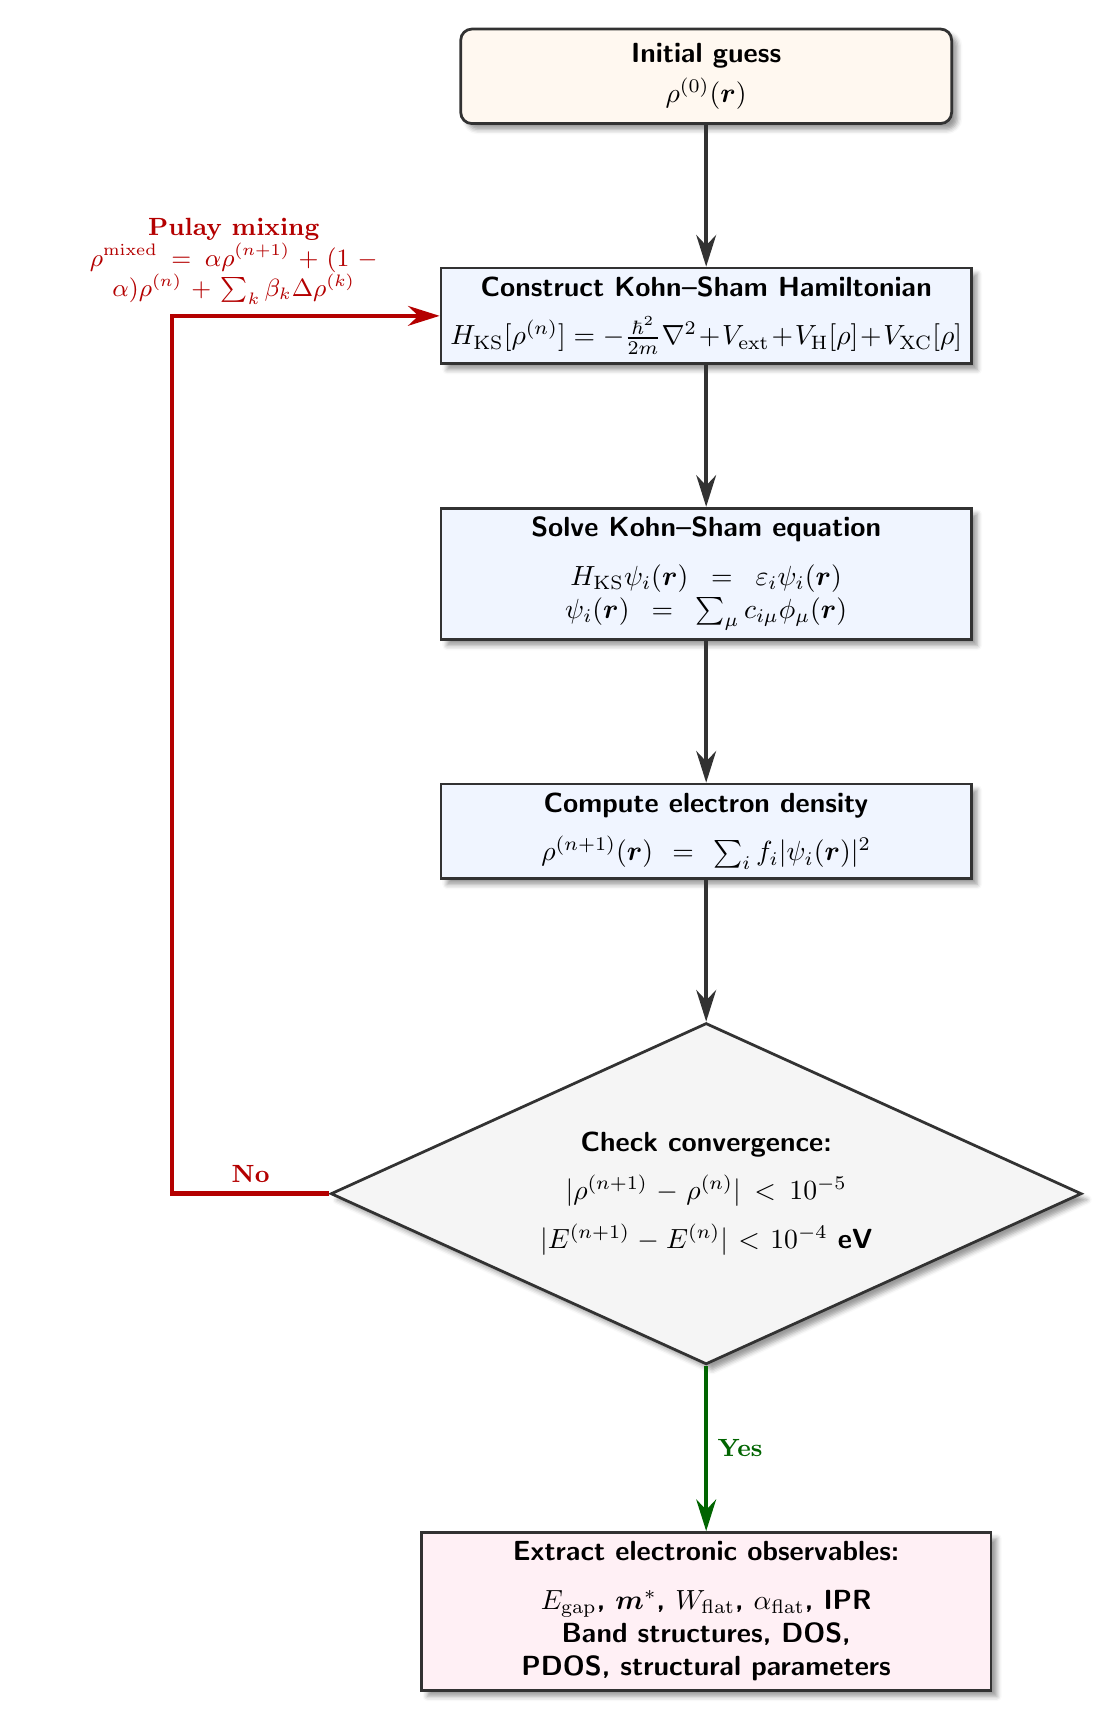
\begin{tikzpicture}[node distance=1.8cm]
% Nodes
\node[startstop, text width=6cm, align=center] (start) {\textbf{Initial guess}\\[0.25em]
$\rho^{(0)}(\boldsymbol{r})$};
\node[block, below=of start] (vks) {\textbf{Construct Kohn--Sham Hamiltonian}\\[0.5em]
$H_{\mathrm{KS}}[\rho^{(n)}] = -\frac{\hbar^2}{2m}\nabla^2 + V_{\mathrm{ext}} + V_{\mathrm{H}}[\rho] + V_{\mathrm{XC}}[\rho]$};
\node[block, below=of vks] (ks) {\textbf{Solve Kohn--Sham equation}\\[0.5em]
$H_{\mathrm{KS}} \psi_i(\boldsymbol{r}) = \varepsilon_i \psi_i(\boldsymbol{r})$\\
$\psi_i(\boldsymbol{r}) = \sum_\mu c_{i\mu} \phi_\mu(\boldsymbol{r})$};
\node[block, below=of ks] (density) {\textbf{Compute electron density}\\[0.5em]
$\rho^{(n+1)}(\boldsymbol{r}) = \sum_i f_i|\psi_i(\boldsymbol{r})|^2$};
\node[decision, below=of density] (check) {
\textbf{Check convergence:}\\[0.5em]
$| \rho^{(n+1)} - \rho^{(n)} | < 10^{-5}$\\[0.5em]
$|E^{(n+1)} - E^{(n)}| < 10^{-4}$ eV
};
\node[finalblock, below=2.1cm of check] (output) {
\textbf{Extract electronic observables:}\\[0.5em]
$E_{\mathrm{gap}}$, $\boldsymbol{m}^*$, $W_{\mathrm{flat}}$, $\alpha_{\mathrm{flat}}$, IPR\\
Band structures, DOS, PDOS, structural parameters
};
% Arrows
\draw[arrow] (start) -- (vks);
\draw[arrow] (vks) -- (ks);
\draw[arrow] (ks) -- (density);
\draw[arrow] (density) -- (check);
\draw[yesarrow] (check) -- node[right, text=yescolor, font=\small\bfseries] {Yes} (output);
% Loop for "No"
\path (check.west) -- ++(-2.0,0) coordinate (left);
\draw[noarrow] (check.west) -- (left) node[midway, above, text=nocolor, font=\small\bfseries] {No} |- (vks.west);
% Mixing label
\node[text=nocolor, font=\small\bfseries, align=center, text width=5cm] at (-6,-2.35) 
  {Pulay mixing\\ $\rho^{\mathrm{mixed}} = \alpha\rho^{(n+1)} + (1-\alpha)\rho^{(n)} + \sum_k \beta_k\Delta\rho^{(k)}$};
\end{tikzpicture}
\end{document}
